\documentclass[12pt]{extarticle}
\usepackage {mathtext}
\usepackage [russian] {babel}
\usepackage {amsmath, caption, geometry, amssymb, graphicx, wrapfig, subfig, derivative}
\usepackage{booktabs}
\usepackage{pgfplots}
\usepackage{float}
\pgfplotsset{compat=1.18}

\pgfplotsset{compat=1.18}

\captionsetup[table]{
	justification=raggedleft,
	singlelinecheck=false,
	labelsep=colon
}
\newcommand{\eds}{\mathcal{E}}

\geometry{left = 2cm, right=1cm, top=15mm, bottom=20mm}

\title{Лабораторная работа №3.7.1. \\ \textbf{Скин-эффект в полом цилиндре}}
\author{Павел Рудачихин, Данила Шеломанов. Б04-507}
\date{13.10.2026}
\begin {document}
\maketitle{}


\section {Аннотация} 
	
	\hspace{4.5mm} Целью настоящей работы является проверка теоретической зависимости ослабления переменного магнитного поля в полом медном цилиндре от частоты и измерение проводимости материала цилиндра.
	
	В основе экспериментального метода лежит пропорциональность магнитного поля внутри соленоида и тока через него, пропорциональность ЭДС индукции амплитуде и частоте переменного магнитного поля, влияние скин-эффекта сердечника на индуктивность катушки.

\section {Теоретическое введение}

	\hspace{4.5mm} При помещении тонкостенного проводящего цилиндра (радиуса $a$ и толщины стенки $h \ll a$) в переменное продольное магнитное поле соленоида в стенках цилиндра индуцируются вихревые токи Фуко, препятствующие проникновению поля внутрь. 
	
	\begin{figure}[h!]
		\centering
		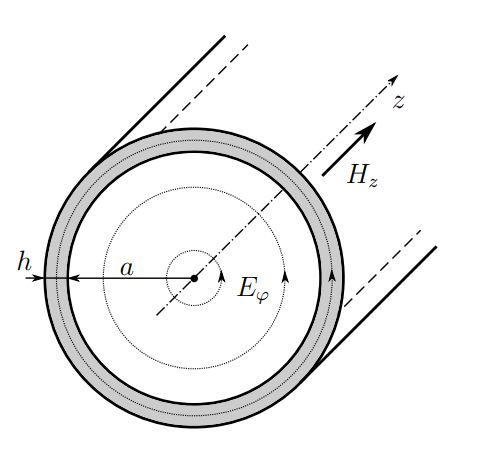
\includegraphics[width=0.3\linewidth]{cilindre}
		\caption{Скин-эффект в полом цилиндре}
		\label{fig:cilindre}
	\end{figure}
	
	Пусть цилиндр достаточно длинный, так что
	в нём можно пренебречь краевыми эффектами. Тогда магнитное поле \textbf{H} всюду направлено по оси системы, а вихревое электрическое поле \textbf{E} перпендикулярно радиусу,
	то есть линии поля образуют соосные окружности (см. рис. 1).
	
	Все величины будем считать колеблющимися по гармоническому закону с некоторой частотой $\omega$, задаваемой частотой колебания тока в соленоиде:
	
	\begin{equation}
		H_z = H(r) e^{i\omega t}, \ \ \ E_\varphi = E(r) e^{i\omega t}
	\end{equation}
	
	
	
	Поскольку внутри цилиндра ток отсутствует, магнитное поле там является однородным $H_z(r, t) = H_1 e^{i\omega t}$, где $H_1$ -- поле на внутренней поверхности цилиндра. С учётом закона электромагнитной индукции имеем
	
	\begin{equation}
		E(r) = - \frac{1}{2}r \mu \mu_0 i \omega H_1 
	\end{equation}
	
	где $\mu$ -- магнитная проницаемость.
	
	Из уравнения диффузии поля
	
	\begin{equation}
		\Delta \textbf{H} = \sigma \mu \mu_0 \pdv{\textbf{H}}{t}, 
	\end{equation}
	
	где $\sigma$ -- проводимость, имеем дифференциальное уравнение для комплексной амплитуды магнитного поля
	
	\begin{equation}
		\odv[2]{H}{x}  = i \omega \sigma \mu \mu_0 H 
	\end{equation}
	
	с граничными условиями $H(0) = H_0$, $H(h) = H_1$, где $H_0$ -- поле на внешней границе цилиндра, равное полю внутри соленоида в отсутствие экрана. Решение этого уравнения имеет вид
	
	\begin{equation}
		H(x)  = Ae^{\alpha x} + B^{-\alpha x} 
	\end{equation}
	
	где подстановкой находим $\alpha = \sqrt{i\omega \sigma \mu \mu_0}$. Введём глубину скин-слоя 
	
	\begin{equation}
		\delta = \sqrt{\frac{2}{\omega \sigma \mu \mu_0}}
	\end{equation}
	
	Используя граничные условия, уравнение (2) и закон Ампера $dH/dx = \sigma E(x)$, получаем
	
	\begin{equation}
		H_1 = \frac{H_0}{\ch(\alpha h) + \frac{1}{2}\alpha a \sh(\alpha h)}
		\label{eq:H1_H0}
	\end{equation}
	
	Предельные случаи:
	
	1. Малые частоты -- толщина скин-слоя превосходит толщину стенки цилиндра, поэтому 
	
	\begin{equation}
		H_1 \approx \frac{H_0}{1 + i \frac{ah}{\delta^2}}; \ \ \ \frac{|H_1|}{|H_0|} = \frac{1}{\sqrt{1 + 0,25(ah\sigma\mu_0\omega)^2}}; \ \ \ \tg \psi = \frac{ah}{\delta^2}
	\end{equation}
	где $\psi$ -- сдвиг фаз между $H_1$ и $H_0$.
	
	2. Высокие частоты -- толщина скин-слоя меньше толщины стенки цилиндра, поэтому 
	
	\begin{equation}
		H_1 \approx \frac{4 H_0 e^{-\alpha h}}{\alpha a}; \ \ \ \frac{|H_1|}{|H_0|} = \frac{2\sqrt{2} \delta}{a} e^{-h/\delta}; \ \ \ \tg \psi = \frac{\pi}{4} + \frac{h}{\delta}
	\end{equation}
	
	В работе отношение амплитуд магнитных полей находится через измеряемые напряжение на внутренней катушке $U \propto \nu |H_1|$ и ток в соленоиде $I \propto |H_0|$:
	\begin{equation}
		\frac{|H_1|}{|H_0|} = c \cdot \frac{U}{\nu I} = c\xi,
		\label{eq:xi}
	\end{equation}
	где калибровочная константа $c$ определяется из условия $|H_1|/|H_0| \to 1$ при $\nu \to 0$.
	
	
	
\section{Описание установки}

	\hspace{4.5mm} В работе используются: генератор звуковой частоты, соленоид, медный трубчатый экран, измерительная катушка, амперметр, вольтметр, осциллограф.
	
	\begin{figure}[h!]
		\centering
		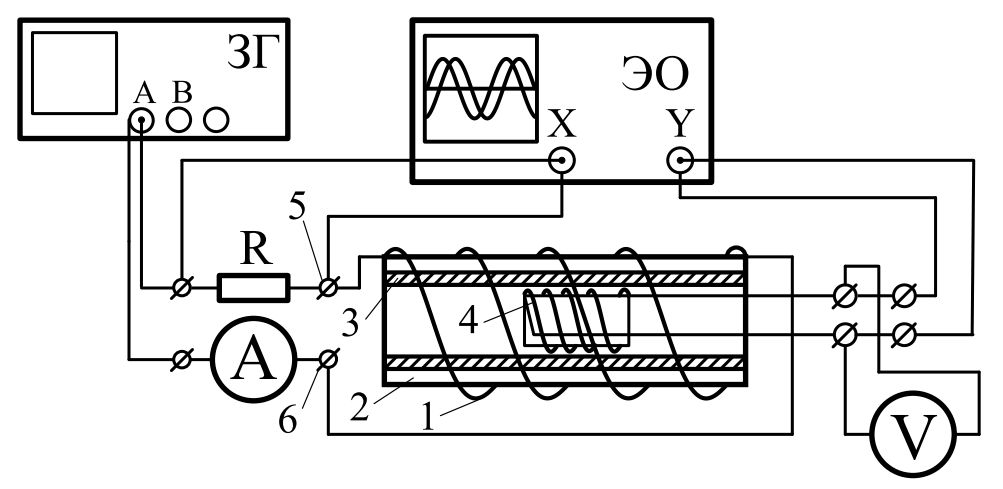
\includegraphics[width=0.7\linewidth]{setup}
		\caption{Схема установки}
		\label{fig:setup}
	\end{figure}
	
	
	С помощью соленоида 1, намотанного на диэлектрический каркас 2, и подключённого к нему генератора звуковой частоты ЗГ создаётся переменное магнитное поле (см. рис. 2). Внутри соленоида расположен медный цилиндрический полый экран 3. Внутри него -- измерительная катушка 4. С помощью амперметра А измеряется действующее значение переменного тока в соленоиде, с помощью вольтметра V -- действующее значение напряжения на измерительной катушке. Для измерения сдвига фаз используется двухканальный осциллограф ЭО. На один его вход подаётся напряжение с резистора R, на другой -- с измерительной катушки. 
	
	Показания вольтметра пропорциональны амплитуде магнитного поля и частоте сигнала: $U \propto |H_1| \nu$. Поле вне экрана пропорционально току в соленоиде $|H_0| \propto I$. Следовательно
	
	\begin{equation}
		\frac{|H_1|}{|H_0|} = C \frac{U}{\nu I}
	\end{equation}
	
	где $C$ определяется при $\nu \rightarrow 0$.
	
	
\section{Результаты и обсуждения}

	Оценим частоту, при которой глубина скин-слоя равна толщине стенки с учётом $\sigma \sim 5\cdot10^7$ См/м:
	
	\begin{equation}
		\nu_h = \frac{1}{\pi \mu_0 \sigma h^2} \approx 2250 \ Гц
	\end{equation}
	
	\subsection{Измерение проводимости через отношение амплитуд}
	
	Результаты измерений в области малых частот ($\nu = 25\text{--}125\text{ Гц}$) представлены в таблице \ref{tab:low_amp}. Введём
	
	\begin{equation}
		\xi = \frac{U}{\nu I} = \xi_0 \frac{|H_1|}{|H_0|}
	\end{equation}
	
	Построим график в координатах $1/\xi^2(\nu^2)$ (см. рис. 3). Аппроксимируем линейной зависимостью. Экстраполируя к $\nu = 0$ находим $1/\xi_0 = (69,13 \pm 0,04)$. По угловому коэффициенту находим 
	\[
	\sigma_1 = (4,452 \pm 0,010)\cdot 10^7\text{ См/м}
	\]
	\begin{figure}[H]
		\centering
		\begin{tikzpicture}
			\begin{axis}[
				width=13cm, height=7.5cm,
				xlabel={$\nu^2$, $\text{Гц}^2$},
				ylabel={$1/\xi^2$, $\text{А}^2\cdot\text{Гц}^2/\text{В}^2$},
				grid=both,
				grid style={line width=.1pt, draw=gray!20},
				major grid style={line width=.2pt,draw=gray!50},
				legend pos=north west,
				xmin=0, xmax=16500,
				ymin=4700, ymax=7600
				]
				\addplot[only marks, mark=*, mark size=2pt, color=blue] coordinates {
					(625, 4906.565) (1225, 4973.776) (2025, 5102.152) (3025, 5282.000)
					(4225, 5500.628) (5625, 5728.484) (7225, 6002.821) (9025, 6299.450)
					(11025, 6662.760) (13225, 7020.046) (15625, 7420.241)
				};
				%\addlegendentry{Экспериментальные точки}
				
				\addplot[domain=0:16000, samples=100, color=red, thick] {0.1682*x + 4779.3};
				%\addlegendentry{Аппроксимация: $y = (0.1682 \pm 0.0007)x + (4779 \pm 5)$}
			\end{axis}
		\end{tikzpicture}
		\caption{График зависимости $1/\xi^2$ от $\nu^2$}
		\label{fig:amp_low}
	\end{figure}
	

	
	\subsection{Измерение проводимости через разность фаз в низкочастотном диапазоне}
	
	В диапазоне частот $\nu = 125\text{--}410\text{ Гц}$  измерялись параметры сдвига сигналов $x$ и $x_0$ (таблица \ref{tab:phase_low}). С учетом сдвига фазы на $\pi/2$ на измерительной катушке тангенс сдвига фазы поля определяется как $\tg\psi = \frac{x}{\sqrt{x_0^2 - x^2}}$.
	
	
	
	\begin{figure}[H]
		\centering
		\begin{tikzpicture}
			\begin{axis}[
				width=13cm, height=7.5cm,
				xlabel={$\nu$, Гц},
				ylabel={$\tg\psi$},
				grid=both,
				grid style={line width=.1pt, draw=gray!20},
				major grid style={line width=.2pt,draw=gray!50},
				legend pos=north west,
				xmin=100, xmax=440,
				ymin=0.7, ymax=2.6
				]
				\addplot[
				only marks, mark=*, mark size=2pt, color=blue,
				error bars/.cd, y dir=both, y explicit
				] coordinates {
					(125, 1.134) +- (0, 0.12)
					(135, 1.237) +- (0, 0.13)
					(145, 1.307) +- (0, 0.14)
					(155, 1.252) +- (0, 0.14)
					(165, 1.333) +- (0, 0.15)
					(175, 1.302) +- (0, 0.15)
					(185, 1.406) +- (0, 0.16)
					(225, 1.423) +- (0, 0.15)
					(245, 1.614) +- (0, 0.18)
					(265, 1.385) +- (0, 0.16)
					(285, 1.480) +- (0, 0.17)
					(315, 1.572) +- (0, 0.19)
					(345, 1.701) +- (0, 0.21)
					(375, 1.826) +- (0, 0.20)
					(410, 2.294) +- (0, 0.35)
				};
				%\addlegendentry{Экспериментальные точки}
				
				\addplot[domain=100:430, samples=100, color=red, thick] {0.004*x + 0.5};
				%\addlegendentry{Аппроксимация: $\tan\psi = 0.00585\nu$}
			\end{axis}
		\end{tikzpicture}
		\caption{График зависимости $\tan\psi(\nu)$ в низкочастотной области}
		\label{fig:phase_low}
	\end{figure}
	
	По коэффициенту наклона прямой $k = \pi a h \sigma \mu_0 = (0,00585 \pm 0,00018)\text{ Гц}^{-1}$ находим проводимость:
	\[
	\sigma_2 = \frac{k}{\pi a h \mu_0} = (4,39 \pm 0,14)\cdot 10^7\text{ См/м}.
	\]
	
	\subsection{Измерение проводимости через разность фаз в высокочастотном диапазоне}
	
	Результаты измерений при высоких частотах ($\nu = 450\text{--}25000\text{ Гц}$) приведены в таблице \ref{tab:phase_high}. По ним строим график в координатах $\psi - \pi/4 = f(\sqrt{\nu})$. 
	
	
	
	\begin{figure}[H]
		\centering
		\begin{tikzpicture}
			\begin{axis}[
				width=13cm, height=7.5cm,
				xlabel={$\sqrt{\nu}$, $\text{Гц}^{1/2}$},
				ylabel={$\psi - \pi/4$, рад},
				grid=both,
				grid style={line width=.1pt, draw=gray!20},
				major grid style={line width=.2pt,draw=gray!50},
				legend pos=north west,
				xmin=0, xmax=170,
				ymin=0, ymax=3.3
				]
				\addplot[only marks, mark=*, mark size=2pt, color=blue] coordinates {
					(21.21, 0.351) (23.45, 0.422) (27.39, 0.540) (30.82, 0.589)
					(38.73, 0.720) (44.72, 0.858) (54.77, 1.036) (63.25, 1.186)
					(77.46, 1.564) (89.44, 1.662) (100.00, 1.763) (122.47, 2.345)
					(141.42, 2.637) (158.11, 2.987)
				};
				%\addlegendentry{Экспериментальные точки}
				
				\addplot[domain=0:165, samples=100, color=red, thick] {0.0191*x};
				%\addlegendentry{Аппроксимация: $\psi - \pi/4 = (0.0191 \pm 0.0006)\sqrt{\nu}$}
			\end{axis}
		\end{tikzpicture}
		\caption{График зависимости $(\psi - \pi/4)$ от $\sqrt{\nu}$ при высоких частотах}
		\label{fig:phase_high}
	\end{figure}
	
	Аппроксимируем прямой с угловым коэффициентом  $\kappa = h\sqrt{\pi\mu_0\sigma} = (0,0191 \pm 0,0006)\text{ Гц}^{-1/2}$ получаем:
	\[
	\sigma_3 = \frac{\kappa^2}{\pi \mu_0 h^2} = (4,11 \pm 0,26)\cdot 10^7\text{ См/м}.
	\]
	
	\subsection{Измерение проводимости через изменение индуктивности}
	
	Данные измерений индуктивности внешней катушки $L(\nu)$ представлены в таблице \ref{tab:inductance}. Определены предельные значения: $L_{\max} = 10,65\text{ мГн}$ и $L_{\min} = 2.91\text{ мГн}$.
	
	
	
	\begin{figure}[H]
		\centering
		\begin{tikzpicture}
			\begin{axis}[
				width=6.8cm, height=6cm,
				xlabel={$\nu$, Гц},
				ylabel={$L$, мГн},
				grid=both,
				grid style={line width=.1pt, draw=gray!20},
				major grid style={line width=.2pt,draw=gray!50},
				xmin=0, xmax=3200,
				ymin=2.5, ymax=10.5,
				title={а) Зависимость $L(\nu)$}
				]
				\addplot[mark=*, mark size=2pt, color=orange!90!black, thick] coordinates {
					(75, 9.5) (100, 8.8) (150, 7.4) (250, 5.5) (300, 4.9)
					(400, 4.1) (500, 3.7) (800, 3.2) (1500, 3.0) (2000, 2.96)
					(2500, 2.94) (3000, 2.93)
				};
			\end{axis}
		\end{tikzpicture}
		\hfill
		\begin{tikzpicture}
			\begin{axis}[
				width=8.2cm, height=6cm,
				xlabel={$\nu^2$, $\text{кГц}^2$},
				ylabel={$(L_{\max}-L)/(L-L_{\min})$},
				grid=both,
				grid style={line width=.1pt, draw=gray!20},
				major grid style={line width=.2pt,draw=gray!50},
				legend pos=north west,
				xmin=0, xmax=0.7,
				ymin=0, ymax=28,
				title={б) Линеаризация}
				]
				\addplot[only marks, mark=*, mark size=2pt, color=blue] coordinates {
					(0.0056, 0.175) (0.0100, 0.314) (0.0225, 0.724) (0.0625, 1.988)
					(0.0900, 2.889) (0.1600, 5.504) (0.2500, 8.797) (0.6400, 25.69)
				};
				\addplot[domain=0:0.66, samples=100, color=red, thick] {36.1*x};
				%\addlegendentry{$y = (36.1 \pm 0.8)x$}
			\end{axis}
		\end{tikzpicture}
		\caption{Зависимость индуктивности от частоты и ее линеаризация}
		\label{fig:inductance}
	\end{figure}
	
	По коэффициенту наклона $k_L = \pi^2 a^2 h^2 \mu_0^2 \sigma^2 = (36,1 \pm 0,8)\cdot 10^{-6}\text{ Гц}^{-2}$ находим:
	\[
	\sigma_4 = \frac{\sqrt{k_L}}{\pi a h \mu_0} = (4,51 \pm 0,05)\cdot 10^7\text{ См/м}.
	\]
	
	\subsection{Отношение магнитных полей во всем диапазоне частот}
	
	На рис. \ref{fig:all_range} приведено  $|H_1|/|H_0|$ во всем исследованном диапазоне частот $\nu = 25\text{--}25000\text{ Гц}$.
	
	\begin{figure}[H]
		\centering
		\begin{tikzpicture}
			\begin{axis}[
				xmode = log,
				width=13.5cm, height=7.5cm,
				xlabel={$\nu$, Гц (логарифмический масштаб)},
				ylabel={$|H_1|/|H_0|$},
				grid=both,
				grid style={line width=.1pt, draw=gray!20},
				major grid style={line width=.2pt,draw=gray!50},
				legend pos=north east,
				xmin=20, xmax=30000,
				ymin=0.001, ymax=1.2
				]
				\addplot[only marks, mark=*, mark size=1.8pt, color=blue] coordinates {
					(25, 0.9869) (35, 0.9802) (45, 0.9676) (55, 0.9512) (65, 0.9321)
					(75, 0.9134) (85, 0.8923) (95, 0.8710) (105, 0.8469) (115, 0.8251)
					(125, 0.8025) (135, 0.7805) (145, 0.7603) (155, 0.7376) (165, 0.7160)
					(175, 0.6951) (185, 0.6744) (205, 0.6363) (225, 0.6039) (245, 0.5698)
					(265, 0.5396) (285, 0.5117) (315, 0.4749) (345, 0.4416) (375, 0.4126)
					(410, 0.3822) (450, 0.3541) (550, 0.2953) (750, 0.2206) (950, 0.1755)
					(1500, 0.1125) (2000, 0.0839) (3000, 0.0555) (4000, 0.0408)
					(6000, 0.0262) (8000, 0.0186) (10000, 0.0142) (15000, 0.0085)
					(20000, 0.0064) (25000, 0.0060)
				};
				\addlegendentry{Экспериментальные значения}
				
				\addplot[only marks, mark=triangle*, mark size=2pt, color=orange!90!black] coordinates {
					(25, 0.9868) (35, 0.9799) (45, 0.9673) (55, 0.9508) (65, 0.9317)
					(75, 0.9102) (85, 0.8869) (95, 0.8622) (105, 0.8367) (115, 0.8107)
					(125, 0.7846) (155, 0.7082) (185, 0.6377) (225, 0.5561) (285, 0.4596)
					(345, 0.3886) (410, 0.3316) (550, 0.2498) (750, 0.1835) (950, 0.1445)
					(1500, 0.0906) (2000, 0.0669) (3000, 0.0428) (4000, 0.0303)
					(6000, 0.0176) (8000, 0.0112) (10000, 0.0075) (15000, 0.0031)
					(20000, 0.0014) (25000, 0.0007)
				};
				\addlegendentry{Теоретические значения}
			\end{axis}
		\end{tikzpicture}
		\caption{Отношение амплитуд магнитных полей $|H_1|/|H_0|(\nu)$ во всем диапазоне частот}
		\label{fig:all_range}
	\end{figure}
		
\section{Выводы}

	\hspace{4mm} Сравнение результатов измерения удельной проводимости меди четырьмя методами приведено в таблице \ref{tab:summary}.
	\begin{table}[H]
		\centering
		\caption{Сравнение результатов определения проводимости меди различными методами}
		\label{tab:summary}
		\begin{tabular}{lccc}
			\toprule
			Метод измерения & $\sigma$, $10^7\text{ См/м}$ & $\Delta\sigma$, $10^7\text{ См/м}$ & $\varepsilon_\sigma$ \\
			\midrule
			1. Отношение амплитуд (низкие частоты) & 4,452 & 0,010 & 0,22\% \\
			2. Разность фаз (низкие частоты)       & 4,26  & 0,09  & 2,1\%  \\
			3. Разность фаз (высокие частоты)      & 4,11  & 0,26  & 6,3\%  \\
			4. Изменение индуктивности соленоида   & 4,51  & 0,05  & 1,1\%  \\
			\bottomrule
		\end{tabular}
	\end{table}
	
	\begin{enumerate}
		\item Все четыре метода дали согласующиеся друг с другом значения удельной проводимости меди в диапазоне $(4,1...4,5)\cdot 10^7\text{ См/м}$. Отличие от табличного значения для чистой электротехнической меди ($\sigma_{\text{табл}} \approx 5.6\cdot 10^7\text{ См/м}$) обусловлено наличием примесей в сплаве исследуемого цилиндра, а также краевыми эффектами (конечной длиной цилиндра и соленоида).
		\item Наиболее точным является метод измерения через отношение амплитуд на низких частотах ($\varepsilon_\sigma = 0.22\%$), поскольку вольтметр и амперметр обеспечивают более высокую точность, чем измерение сдвига сигнала на экране осциллографа.
		\item Основной источник погрешности измерений -- определение сдвига сигнала на экране осциллографа.
	\end{enumerate}
	
	
\newpage
\section{Приложение}

	\begin{table}[h!]
		\caption{Параметры установки}
		\centering
		\begin{tabular}{|r|c|}
			\hline
			Параметр & Значение \\
			\hline
			Наружный диаметр, $2(a + h)$ & 45 мм  \\
			Толщина стенки, $h$ & 1,5 мм  \\
			Содержание меди, $C_{Cu}$ &  0,995 \\
			Содержание кислорода, $C_{O_2}$ & 0,0008 \\
			\hline
		\end{tabular}
	\end{table}
	
		\begin{table}[H]
		\centering
		\caption{Данные измерений при малых частотах ($\nu = 25\text{--}125\text{ Гц}$)}
		\label{tab:low_amp}
		\begin{tabular}{cccccc}
			\toprule
			$\nu$, Гц & $I$, мА & $U$, мВ & $\xi = \frac{U}{\nu I}$, $\text{В}/(\text{А}\cdot\text{Гц})$ & $\nu^2$, $\text{Гц}^2$ & $1/\xi^2$, $(\text{А}\cdot\text{Гц}/\text{В})^2$ \\
			\midrule
			25  & 448.3 & 160 & 0.014276 & 625   & 4906.57 \\
			35  & 443.3 & 220 & 0.014179 & 1225  & 4973.78 \\
			45  & 438.1 & 276 & 0.013997 & 2025  & 5102.15 \\
			55  & 432.1 & 327 & 0.013759 & 3025  & 5282.00 \\
			65  & 425.6 & 373 & 0.013483 & 4225  & 5500.63 \\
			75  & 418.8 & 415 & 0.013212 & 5625  & 5728.48 \\
			85  & 412.0 & 452 & 0.012907 & 7225  & 6002.82 \\
			95  & 405.2 & 485 & 0.012599 & 9025  & 6299.45 \\
			105 & 398.8 & 513 & 0.012251 & 11025 & 6662.76 \\
			115 & 392.7 & 539 & 0.011935 & 13225 & 7020.05 \\
			125 & 386.6 & 561 & 0.011609 & 15625 & 7420.24 \\
			\bottomrule
		\end{tabular}
	\end{table}
	
	
\begin{table}[H]
	\centering
	\caption{Данные измерений амплитуды и фазы при $\nu = 125\text{--}410\text{ Гц}$}
	\label{tab:phase_low}
	\begin{tabular}{cccccc}
		\toprule
		$\nu$, Гц & $I$, мА & $U$, мВ & $x$, дел. & $x_0$, дел. & $\tg\psi = \frac{x}{\sqrt{x_0^2 - x^2}}$ \\
		\midrule
		125 & 385.0 & 559 & 3.0 & 4.0 & 1.134 \\
		135 & 379.4 & 579 & 2.8 & 3.6 & 1.237 \\
		145 & 374.1 & 596 & 2.7 & 3.4 & 1.307 \\
		155 & 369.4 & 611 & 2.5 & 3.2 & 1.252 \\
		165 & 365.1 & 624 & 2.4 & 3.0 & 1.333 \\
		175 & 361.1 & 635 & 2.3 & 2.9 & 1.302 \\
		185 & 357.2 & 645 & 2.2 & 2.7 & 1.406 \\
		205 & 350.6 & 662 & 4.2 & 4.8 & 1.807 \\
		225 & 344.0 & 676 & 3.6 & 4.4 & 1.423 \\
		245 & 339.9 & 686 & 3.4 & 4.0 & 1.614 \\
		265 & 335.6 & 694 & 3.0 & 3.7 & 1.385 \\
		285 & 331.9 & 700 & 2.9 & 3.5 & 1.480 \\
		315 & 327.0 & 707 & 2.7 & 3.2 & 1.572 \\
		345 & 322.9 & 712 & 2.5 & 2.9 & 1.701 \\
		375 & 319.0 & 714 & 2.3 & 2.7 & 1.626 \\
		410 & 315.6 & 716 & 2.2 & 2.4 & 2.294 \\
		\bottomrule
	\end{tabular}
\end{table}

\begin{table}[H]
	\centering
	\caption{Данные измерений при высоких частотах ($\nu = 450\text{--}25000\text{ Гц}$)}
	\label{tab:phase_high}
	\begin{tabular}{cccccccc}
		\toprule
		$\nu$, Гц & $\sqrt{\nu}$, $\text{Гц}^{1/2}$ & $I$, мА & $U$, мВ & $x$, дел. & $x_0$, дел. & $\psi - \pi/4$, рад & $|H_1|/|H_0| = c\xi$ \\
		\midrule
		450   & 21.21  & 311.0 & 717 & 5.0 & 5.5 & 0.351 & 0.3541 \\
		550   & 23.45  & 303.0 & 712 & 4.2 & 4.5 & 0.422 & 0.2953 \\
		750   & 27.39  & 288.7 & 691 & 3.2 & 3.3 & 0.540 & 0.2206 \\
		950   & 30.82  & 274.4 & 662 & 5.1 & 5.2 & 0.589 & 0.1755 \\
		1500  & 38.73  & 234.0 & 571 & 3.2 & 3.4 & 0.720 & 0.1125 \\
		2000  & 44.72  & 202.8 & 492 & 4.6 & 5.0 & 0.858 & 0.0839 \\
		3000  & 54.77  & 154.0 & 371 & 2.9 & 3.4 & 1.036 & 0.0555 \\
		4000  & 63.25  & 122.3 & 289 & 2.1 & 2.4 & 1.186 & 0.0408 \\
		6000  & 77.46  & 84.6  & 192 & 3.0 & 4.2 & 1.564 & 0.0262 \\
		8000  & 89.44  & 63.6  & 137 & 4.0 & 6.2 & 1.662 & 0.0186 \\
		10000 & 100.00 & 50.0  & 103 & 2.8 & 4.9 & 1.763 & 0.0142 \\
		15000 & 122.47 & 30.2  & 56  & 2.6 & 6.6 & 2.345 & 0.0085 \\
		20000 & 141.42 & 18.8  & 35  & 1.4 & 5.1 & 2.637 & 0.0064 \\
		25000 & 158.11 & 10.6  & 23  & 1.5 & 9.5 & 2.987 & 0.0060 \\
		\bottomrule
	\end{tabular}
\end{table}

\begin{table}[H]
	\centering
	\caption{Зависимость индуктивности соленоида $L$ от частоты $\nu$}
	\label{tab:inductance}
	\begin{tabular}{cccc|cccc}
		\toprule
		$\nu$, Гц & $\nu^2$, $\text{кГц}^2$ & $L$, мГн & $\frac{L_{\max}-L}{L-L_{\min}}$ & $\nu$, Гц & $\nu^2$, $\text{кГц}^2$ & $L$, мГн & $\frac{L_{\max}-L}{L-L_{\min}}$ \\
		\midrule
		75   & 0.0056 & 9.50 & 0.175 & 800  & 0.6400 & 3.20 & 25.69 \\
		100  & 0.0100 & 8.80 & 0.314 & 1500 & 2.2500 & 3.00 & 85.00 \\
		150  & 0.0225 & 7.40 & 0.724 & 2000 & 4.0000 & 2.96 & 153.8 \\
		250  & 0.0625 & 5.50 & 1.988 & 2500 & 6.2500 & 2.94 & 257.0 \\
		300  & 0.0900 & 4.90 & 2.889 & 3000 & 9.0000 & 2.93 & 386.0 \\
		400  & 0.1600 & 4.10 & 5.504 &      &        &      &       \\
		500  & 0.2500 & 3.70 & 8.797 &      &        &      &       \\
		\bottomrule
	\end{tabular}
\end{table}


\end {document}